\documentclass[11pt]{article}
\usepackage[margin = 1in]{geometry}
\usepackage{amsmath}
\usepackage{amssymb}
\usepackage{amsthm}
\usepackage{graphicx}
\usepackage{enumitem}
\usepackage{url}
\usepackage[parfill]{parskip}
\usepackage{listings}
\usepackage{caption}
\usepackage{subcaption}
\usepackage[utf8]{inputenc}
\usepackage{pdfpages}
\usepackage{xcolor}
\definecolor{codegreen}{rgb}{0,0.6,0}
\definecolor{codegray}{rgb}{0.5,0.5,0.5}
\definecolor{codepurple}{rgb}{0.58,0,0.82}
\definecolor{backcolour}{rgb}{0.95,0.95,0.92}
\lstdefinestyle{mystyle}{
	backgroundcolor=\color{backcolour},   
	commentstyle=\color{codegreen},
	keywordstyle=\color{magenta},
	numberstyle=\tiny\color{codegray},
	stringstyle=\color{codepurple},
	basicstyle=\ttfamily\footnotesize,
	breakatwhitespace=false,         
	breaklines=true,                 
	captionpos=b,                    
	keepspaces=true,                 
	numbers=left,                    
	numbersep=5pt,                  
	showspaces=false,                
	showstringspaces=false,
	showtabs=false,                  
	tabsize=2
}
\lstset{style=mystyle}
\newcommand{\skipline}{\vspace{\baselineskip}}
\newcommand{\spacer}{\noalign{\medskip}}
\newcommand{~}{\sim}
\newcommand{\approches}{\rightarrow}
\newcommand{\qarrow}{\quad \rightarrow \quad}
\newcommand{\qqarrow}{\qquad \rightarrow \qquad}
\newcommand{\qqtext}[1]{\qquad \text{ #1 } \qquad}
\newcommand{\pard}[2]{\frac{\partial #1}{\partial #2}}
\newcommand{\answer}[1]{\textbf{\boldmath #1}}
\newenvironment{problem}[1]{\textbf{Problem #1: }}{\newpage}

\begin{document}
	
	\begin{center}
		\textbf{Homework 6} \\
		\textbf{Partial Differential Equations} \\
		\textbf{Math 533} \\
		\textbf{Stephen Giang RedID: 823184070} \\
		\skipline \skipline
	\end{center}

	\begin{problem}{1 Exercise 4.4.1}
		Consider vibrating strings of uniform density $\rho_0$ and tension $T_0$
		\begin{enumerate}[label = (\alph*)]
			\item What are the natural frequencies of a vibrating string of length $L$ fixed at both ends?
			\\ \\
			Notice the linear combination of all product solutions:
			\[u(x,t) = \sum_{n=1}^{\infty} \left( A_n\sin \frac{n\pi x}{L}\cos\frac{n\pi c x}{L} + B_n\sin \frac{n\pi x}{L}\sin\frac{n\pi c x}{L} \right) \] 
			Notice that the circular frequency is:
			\[\omega = \frac{n\pi c}{L} \quad c = \sqrt{\frac{T_0}{\rho_0}}\]
			which is measured in $2\pi$ units of time. The natural frequency is simply this circular frequency in cycles per second:
			\[f = \frac{\omega}{2\pi} = \frac{nc}{2L}\]
			\item What are the natural frequencies of a vibrating string of length $H$, which is fixed at $x = 0$ and ``free'' at the other end [i.e., $\partial u / \partial x (H,t) = 0$]? Sketch a few modes of vibration as in Fig. 4.1.
			\\ \\
			Notice the following from the given information:
			\[u(x,t) = \phi(x)G(t) \qquad \phi(0) = 0 \qquad \phi'(H) = 0\]
			Solving this, we get:
			\[\phi = c_1\cos \sqrt{\lambda}x + c_2\sin \sqrt{\lambda}x \qquad \phi' = -c_1\sqrt{\lambda}\sin \sqrt{\lambda}x + c_2\sqrt{\lambda}\cos \sqrt{\lambda}x\]
			Notice the following from the boundary conditions:
			\[\phi(0) = c_1 = 0 \qqarrow \phi'(H) = c_2\sqrt{\lambda}\cos \sqrt{\lambda}H\]
			We get the following from the non trivial solution:
			\[\lambda = \left( \frac{(2n - 1)\pi}{2H}\right) ^2\]
			From here, we get the circular and natural frequency:
			\[\omega = \frac{(2n-1)\pi c}{2H} \qquad f = \frac{\omega}{2\pi} = \frac{(2n-1)c}{4H} \qquad c = \sqrt{\frac{T_0}{\rho_0}}\]
			\newpage
			\begin{figure}[h!]
				\centering
				\begin{subfigure}{.3\linewidth}
					\centering
					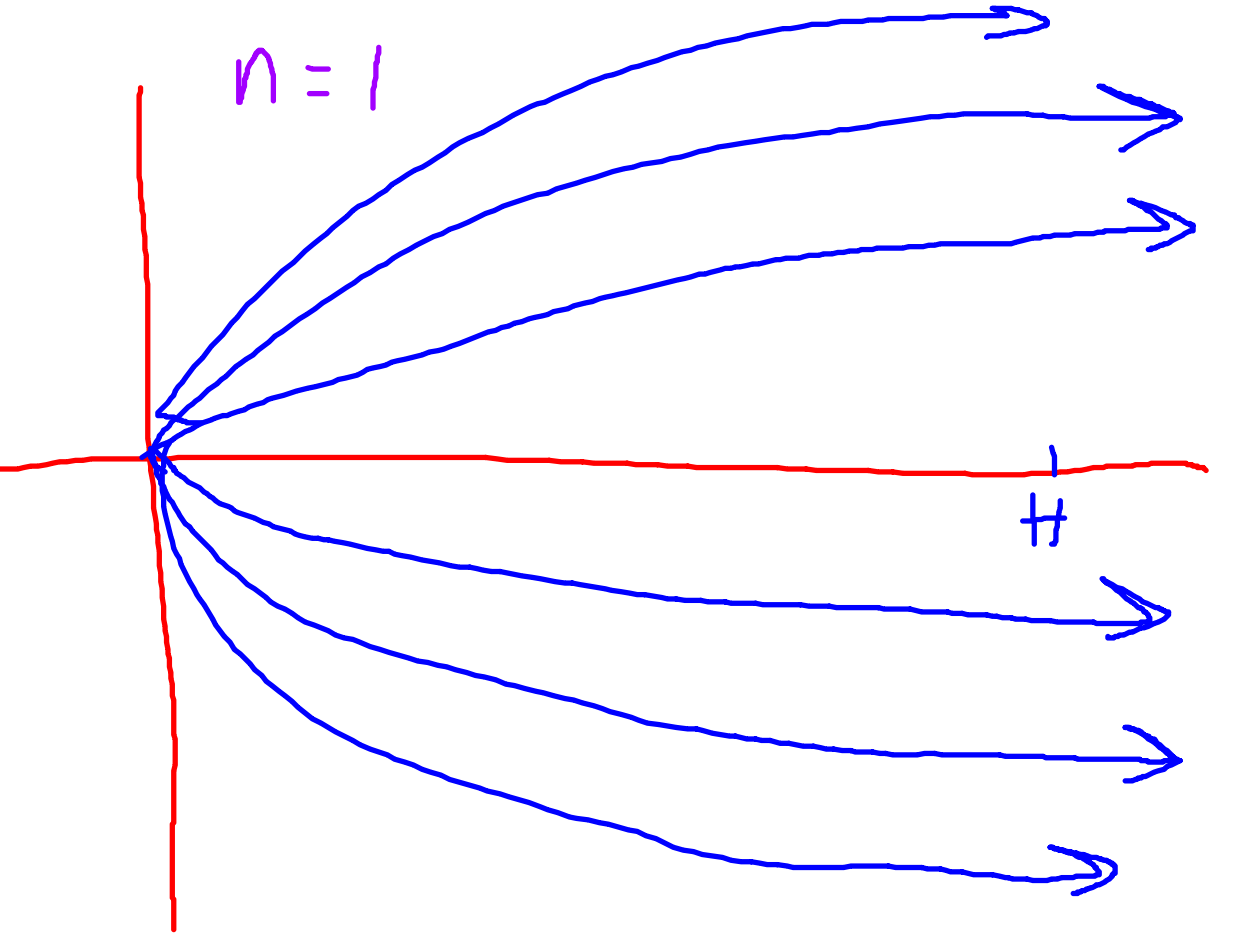
\includegraphics[height=3cm]{n1.png}
				\end{subfigure}
				\begin{subfigure}{.3\linewidth}
					\centering
					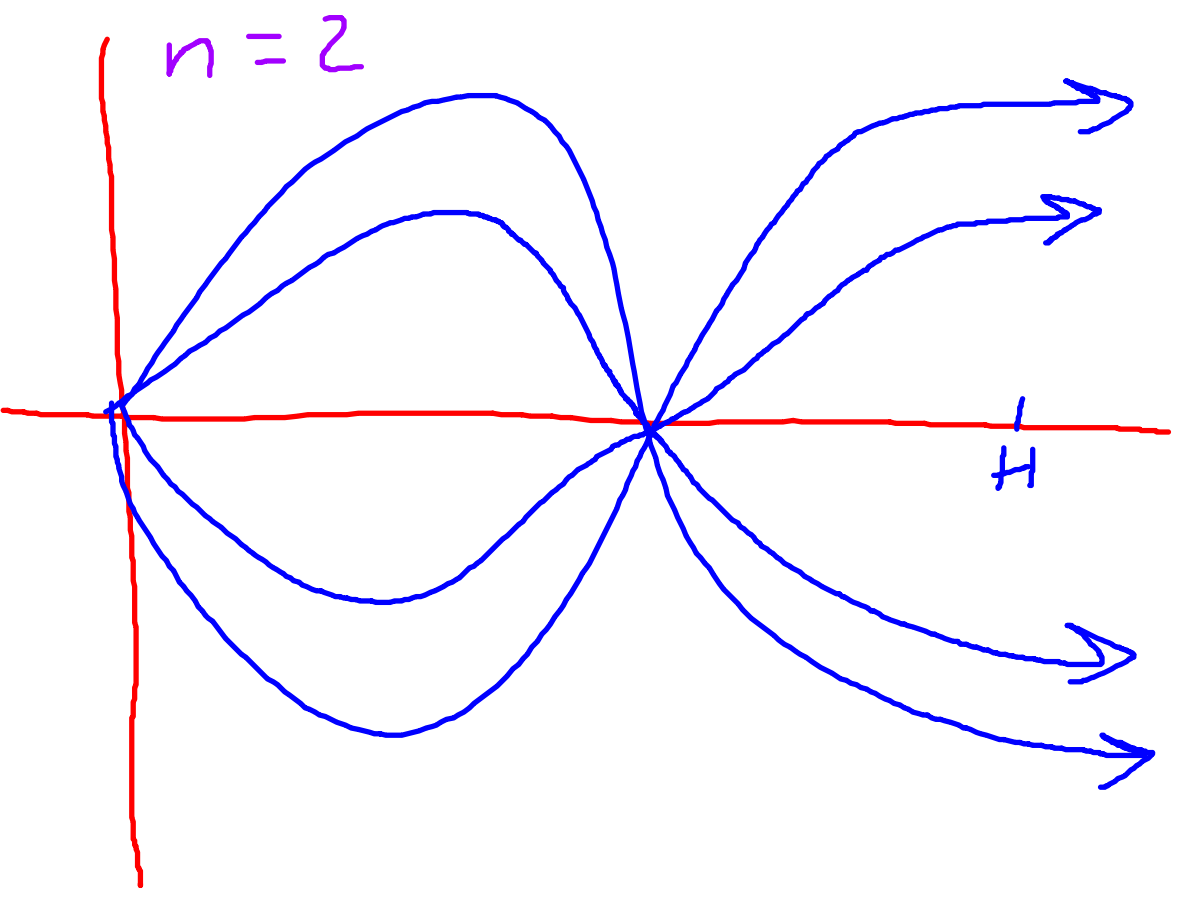
\includegraphics[height=3cm]{n2.png}
				\end{subfigure}
				\begin{subfigure}{.3\linewidth}
					\centering
					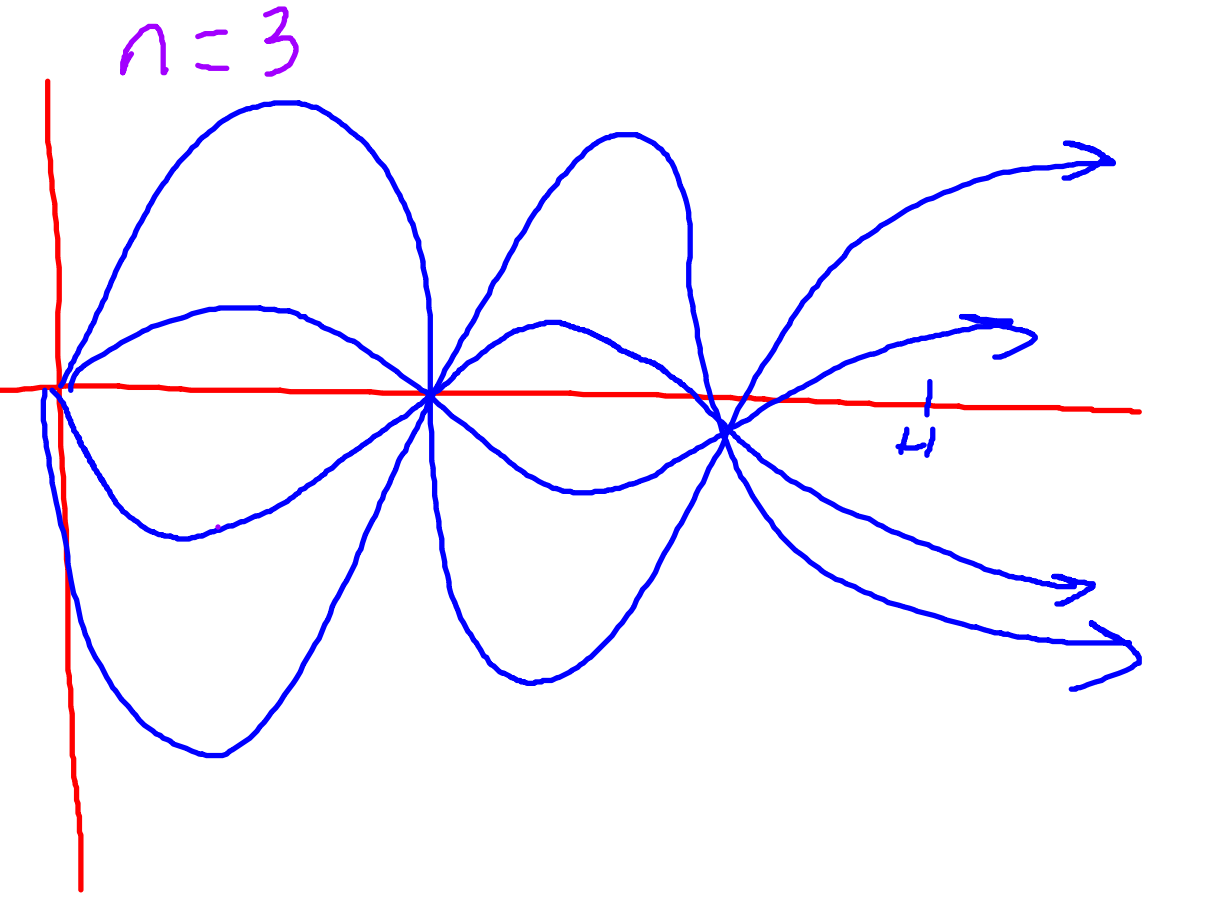
\includegraphics[height=3cm]{n3.png}
				\end{subfigure}
			\end{figure}
			\item Show that the modes of vibration for the \textit{odd} harmonics (i.e., $n = 1, 3, 5,...$) of part (a) are identical to modes of part (b) if $H = L/2$. Verify that their natural frequencies are the same. Briefly explain using symmetry arguments.
			\\ \\
			Notice $u(x,t)$ from part (a) for $n = 2k - 1$:
			\[u(x,t) = \sum_{k=1}^{\infty} \left( A_{2k-1}\sin \frac{(2k-1)\pi x}{L}\cos\frac{(2k-1)\pi c x}{L} + B_{2k-1}\sin \frac{(2k-1)\pi x}{L}\sin\frac{(2k-1)\pi c x}{L} \right) \]
			\\ \\
			Notice $u(x,t)$ from part (b) for $2H = L$:
			\[u(x,t) = \sum_{n=1}^{\infty} \left( A_{2n-1}\sin \frac{(2n-1)\pi x}{L}\cos\frac{(2n-1)\pi c x}{L} + B_{2n-1}\sin \frac{(2n-1)\pi x}{L}\sin\frac{(2n-1)\pi c x}{L} \right) \]
		\end{enumerate}
		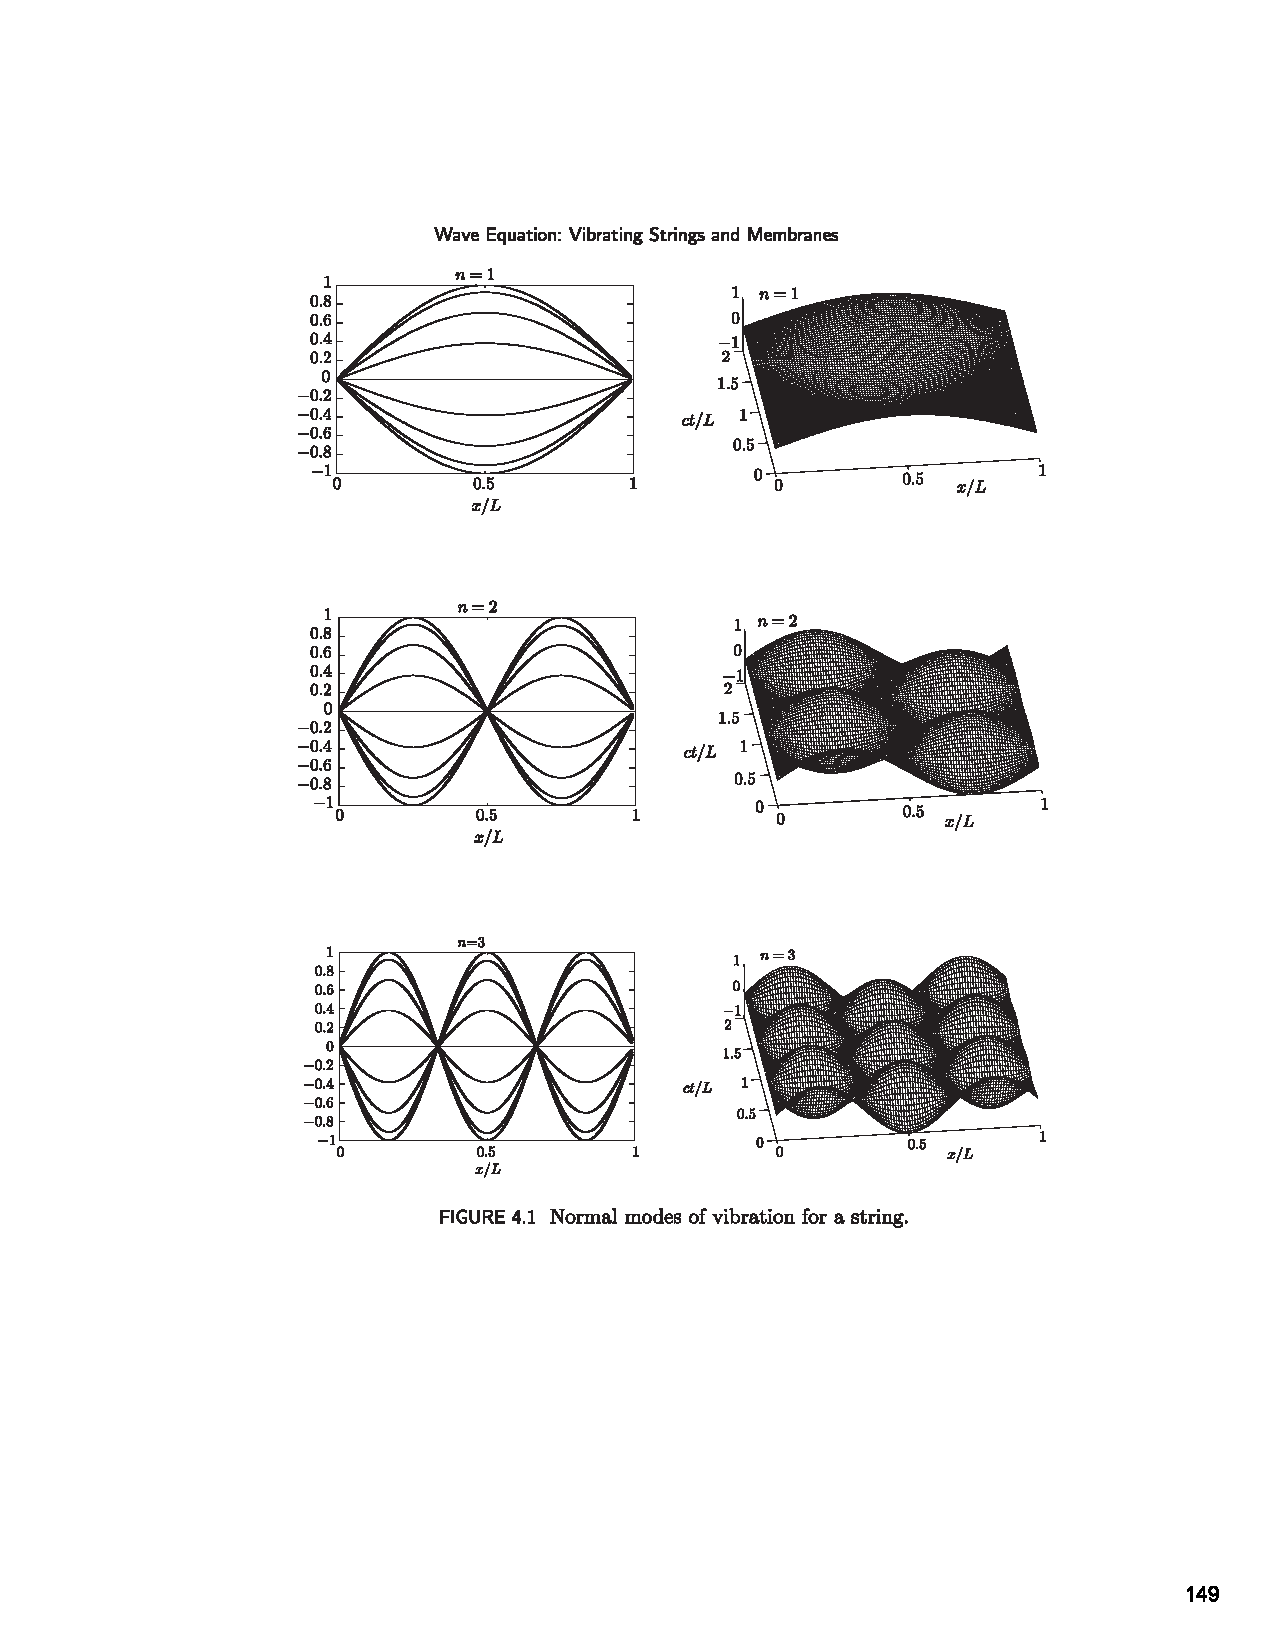
\includepdf{fig41}
	\end{problem}

	\begin{problem}{2 Exercise 4.4.9}
		From (4.1), derive conservation of energy for a vibrating string,
		\[\frac{dE}{dt} = c^2 \pard{u}{x}\pard{u}{t} \bigg|_0^L, \tag{4.15}\]
		where the total energy $E$ is the sum of the kinetic energy, defined by $\int_{0}^{L}\frac{1}{2}\left(\pard{u}{t}\right)^2\,dx$, and the potential energy, defined by $\int_{0}^{L}\frac{c^2}{2}\left(\pard{u}{x}\right)^2\,dx$
		\\ \\
		Notice equation (4.1) as stated in the problem given:
		\[\pard{^2u}{t^2} = c^2\pard{^2u}{x^2}\]
		Notice the equation for total energy, calculated from the sum of kinetic and potential energy.
		\begin{align*}
			E &= KE + PE \\
			&= \int_{0}^{L}\frac{1}{2}\left(\pard{u}{t}\right)^2dx + \int_{0}^{L}\frac{c^2}{2}\left(\pard{u}{x}\right)^2dx
		\end{align*}
		Now notice, when we take the derivative of the total energy:
		\begin{align*}
			\frac{dE}{dt} &= \frac{d}{dt}\int_{0}^{L}\frac{1}{2}\left(\pard{u}{t}\right)^2dx + \frac{d}{dt}\int_{0}^{L}\frac{c^2}{2}\left(\pard{u}{x}\right)^2dx \\
			&= \int_{0}^{L}\frac{1}{2}\frac{d}{dt}\left(\left(\pard{u}{t}\right)^2\right)dx + \frac{d}{dt}\int_{0}^{L}\frac{c^2}{2}\frac{d}{dt}\left(\left(\pard{u}{x}\right)^2\right)dx \\
			&= \int_{0}^{L} \pard{u}{t} \left(\pard{^2u}{t^2}\right)dx + \int_{0}^{L} c^2 \pard{u}{x} \left(\pard{u}{t\partial x}\right)dx \\
			&= \int_{0}^{L} \pard{u}{t} \left(c^2 \pard{^2u}{x^2}\right)dx + \int_{0}^{L} c^2 \pard{u}{x} \left(\pard{u}{t\partial x}\right)dx \\
			&= c^2 \int_{0}^{L} \pard{u}{t} \left(\pard{^2u}{x^2}\right) + \pard{u}{x} \left(\pard{u}{t\partial x}\right)\,dx \\
			&= c^2 \int_{0}^{L} \pard{}{x} \left(\pard{u}{t}\pard{u}{x}\right)\,dx \\
			&= c^2 \pard{u}{x}\pard{u}{t} \bigg|_0^L
		\end{align*}
	\end{problem}

	\begin{problem}{3 Exercise 4.4.10}
		What happens to the total energy E of a vibrating string (see Exercise 4.9)
		Using the result from part (a):
		\[\frac{dE}{dt} = c^2 \pard{u}{x}\pard{u}{t} \bigg|_0^L = c^2 \left(\pard{u(L,t)}{x}\pard{u(L,t)}{t} - \pard{u(0,t)}{x}\pard{u(0,t)}{t}\right)\]
		\begin{enumerate}[label = (\alph*)]
			\item If $u(0, T) = 0$ and $u(L, t) = 0$?
			\\ \\
			With our given boundary conditions, we get the following:
			\[\pard{u(0,t)}{t} = 0 \qquad \pard{u(L,t)}{t} = 0 \]
			Thus, we get with those boundary conditions, we get an insulated system with no change in total energy:
			\[\frac{dE}{dt} = 0\]
			\item If $\pard{u}{x}(0, t) = 0$ and $u(L, t) = 0$?
			\\ \\
			With our given boundary conditions, we get the following:
			\[\pard{u(L,t)}{t} = 0 \]
			Thus, we get with those boundary conditions, we get an insulated system with no change in total energy:
			\[\frac{dE}{dt} = 0\]
			\item If $u(0, t) = 0$ and $\pard{u}{x}(L, t) = -\gamma u(L, t) \text{ with } \gamma > 0$?
			\\ \\
			With our given boundary conditions, we get the following:
			\[\pard{u(0,t)}{t} = 0 \]
			Thus, we get with those boundary conditions, we get an non-insulated system with a loss in total energy:
			\[\frac{dE}{dt} = c^2\left(-\gamma u(L,t)\pard{u(L,t)}{t}\right) = -c^2\gamma u(L,t)\pard{u(L,t)}{t} < 0 \]
			\item If $\gamma < 0$ in part (c)?
			\\ \\
			If $\gamma < 0$ in part (c), we would get that $\frac{dE}{dt} > 0$, which would lead into a gain in total energy.
		\end{enumerate}
	\end{problem}

	\begin{problem}{4 Exercise 5.3.2}
		Consider
		\[\rho \pard{^2u}{t^2} = T_0\pard{^2u}{x^2} + \alpha u + \beta \pard{u}{t}\]
		\begin{enumerate}[label = (\alph*)]
			\item Give a brief physical interpretation. What signs must $\alpha$ and $\beta$ have to be physical?
			\item Allow $\rho$, $\alpha$, and $\beta$ to be functions of $x$. Show that separation of variables works only if $\beta = c\rho$, where $c$ is a constant.
			\\ \\
			Let $u(x,t) = \phi(x)G(t)$, so we can get the following:
			\begin{align*}
				\rho \phi(x)G''(t) &= T_0\phi''(x)G(t) + \alpha\phi(x)G(t)  + \beta\phi(x)G'(t) \\
				\rho \phi(x) (G''(t)) &= G(t) \left( T_0\phi''(x) + \alpha\phi(x)  + \beta\phi(x)\frac{G'(t)}{G(t)}\right) \\
				\frac{G''}{G} &= \frac{T_0}{\rho}\frac{\phi''}{\phi} + \frac{\alpha}{\rho}  + \frac{\beta}{\rho}\frac{G'}{G} \\
				\frac{G''}{G} - \frac{\beta}{\rho}\frac{G'}{G} &= \frac{T_0}{\rho}\frac{\phi''}{\phi} + \frac{\alpha}{\rho} 
			\end{align*}
			From here we can see, we can no longer separate these two equations.  With $\beta$ on the same side of the equation as $G(t)$, the only way to separate the variables is for $\beta = c\rho$, giving us the following:
			\[\frac{G''}{G} - c\frac{G'}{G} = \frac{T_0}{\rho}\frac{\phi''}{\phi} + \frac{\alpha}{\rho} = -\lambda\]
			\newpage
			\item If $\beta = c\rho$, show that the spatial equation is a Sturm–Liouville differential equation. Solve the time equation.
			\\ \\
			Notice the spatial equation:
			\[\frac{1}{\rho} \left( T_0 \frac{\phi''}{\phi} + \alpha\right) = -\lambda \qqarrow T_0 \phi'' + (\lambda\rho + \alpha)\phi = 0 \]
			Notice that this is a Sturm–Liouville differential equation with
			\[p(x) = T_0, \qquad \sigma(x) = \rho(x), \qquad q(x) = \alpha(x)\]
			Notice the time equation:
			\[\frac{G''}{G} - c\frac{G'}{G} = -\lambda \qqarrow G'' - cG' + \lambda G = 0\]
			Notice from the characteristic equation, we get: 
			\[r = \frac{c \pm \sqrt{c^2 - 4\lambda}}{2}\]
			From here, we can see the following solutions:
			\begin{enumerate}[label = (\alph*)]
				\item Let $c^2 = 4\lambda$: we get the following solution:
				\[G = \left(c_1 + c_2\,t\right)e^{ct/2}\]
				\item Let $c^2 < 4\lambda$: we get the following solution:
				\[G = e^{c/2}\left(c_1\cos\left(\frac{\sqrt{|c^2 - 4\lambda|}}{2}\,t\right) + c_2\sin\left(\frac{\sqrt{|c^2 - 4\lambda|}}{2}\,t\right) \right)\]
				\item Let $c^2 > 4\lambda$: we get the following solution:
				\[G = c_1e^{\frac{c + \sqrt{c^2 - 4\lambda}}{2}} + c_2e^{\frac{c - \sqrt{c^2 - 4\lambda}}{2}}\]
			\end{enumerate}
		\end{enumerate}
	\end{problem}

	\begin{problem}{5 Exercise 5.3.3}
		Consider the non-Sturm–Liouville differential equation
		\[\frac{d^2\phi}{dx^2} + \alpha(x)\frac{d\phi}{dx} + \left[\lambda\beta(x) + \gamma(x)\right]\phi = 0.\]
		Multiply this equation by $H(x)$. Determine $H(x)$ such that the equation may be
		reduced to the standard Sturm–Liouville form:
		\[\frac{d}{dx}\left[p(x)\frac{d\phi}{dx}\right] + \left[\lambda\sigma(x) + q(x)\right]\phi = 0. \]
		Given $\alpha(x), \beta(x)$, and $\gamma(x)$, what are $p(x), \sigma(x)$, and $q(x)$?
		\\ \\
		Notice the result by multiplying the equation by $H(x)$:
		\[H(x)\frac{d^2\phi}{dx^2} + H(x)\alpha(x)\frac{d\phi}{dx} + \left[\lambda H(x)\beta(x) + H(x)\gamma(x)\right]\phi = 0.\]
		Now we can notice that if we let the following be true, we can reduce the non-Sturm–Liouville differential equation into the standard Sturm–Liouville form
		\[p(x) = H(x) \qquad p'(x) = H'(x) = H(x)\alpha(x) \qquad \sigma(x) = H(x)\beta(x) \qquad q(x)=H(x)\gamma(x)\]
		Now we can write the first two terms into the derivative of $H(x)\phi'(x)$
		\[\frac{d}{dx}\left(H(x)\frac{d\phi}{dx}\right) + \left[\lambda H(x)\beta(x) + H(x)\gamma(x)\right]\phi = 0.\]
		Now we simply substitute to get the final result:
		\[\frac{d}{dx}\left[p(x)\frac{d\phi}{dx}\right] + \left[\lambda\sigma(x) + q(x)\right]\phi = 0. \]
		Now, given $\alpha(x), \beta(x), \gamma(x)$, we can calculate $H(x)$:
		\[H'(x) = H(x)\alpha(x) \qqarrow H(x) = Ce^{\int \alpha(x)\,dx}\]
		Thus we get the following for $p(x), \sigma(x)$, and $q(x)$:
		\[p(x) = Ce^{\int \alpha(x)\,dx} \qquad \sigma(x) = Ce^{\int \alpha(x)\,dx}\beta(x) \qquad q(x)=Ce^{\int \alpha(x)\,dx}\gamma(x)\]
	\end{problem}

	\begin{problem}{6 Exercise 5.3.9}
		Consider the eigenvalue problem
		\[x^2\frac{d^2\phi}{dx^2} + x\frac{d\phi}{dx} + \lambda \phi = 0 \text{ with } \phi(1) = 0 \text{ and } \phi(b) = 0. \tag{3.10}\]
		\begin{enumerate}[label = (\alph*)]
			\item Show that multiplying by $1/x$ puts this in the Sturm–Liouville form. (This multiplicative factor is derived in Exercise 3.3.)
			\\ \\
			Notice the Sturm–Liouville form:
			\[\frac{d}{dx}\left[p(x)\frac{d\phi}{dx}\right] + \left[\lambda\sigma(x) + q(x)\right]\phi = 0.\]
			Now we multiply the equation by $1/x$:
			\[x\frac{d^2\phi}{dx^2} + \frac{d\phi}{dx} + \lambda\frac{1}{x}\phi = 0\]
			From here, we can write this in the Sturm–Liouville form:
			\[\frac{d}{dx}\left[x\frac{d\phi}{dx}\right] + \left[\lambda \frac{1}{x} + 0\right]\phi = 0 \qqarrow \frac{d}{dx}\left[x\frac{d\phi}{dx}\right] + \frac{\lambda}{x}\phi = 0\]
			In this case, we have the following:
			\[p(x) = x \qquad \sigma(x) = \frac{1}{x} \qquad q(x) = 0\]
			\item Show that $\lambda \geq 0$.
			\\ \\
			Notice, we can use the Rayleigh quotient to find $\lambda$:
			\[\lambda = \frac{-p(x)\phi(x)\phi'(x)\bigg|_a^b + \int_{a}^{b} \bigg[p(x)\left(\frac{d\phi}{dx}\right)^2 - q(x)\phi^2(x)\bigg]\,dx}{\int_{a}^b \phi^2(x)\sigma(x)\,dx}\]
			Substituting our parameters and using our BC's, we get:
			\[\lambda = \int_{1}^{b} x\left(\frac{d\phi}{dx}\right)^2\,dx \bigg/ \int_{1}^b \frac{\phi^2(x)}{x}\,dx \]
			Notice that in the interval $x = [1,b], x > 0$, and at all values of $x, (\phi''(x))^2 \geq 0 \text{ and } \phi^2(x) \geq 0$.  Thus we get the following:
			\[\lambda = \int_{1}^{b} x\left(\frac{d\phi}{dx}\right)^2\,dx \bigg/ \int_{1}^b \frac{\phi^2(x)}{x}\,dx \geq 0\]
			\newpage
			\item Since (3.10) is an equidimensional equation, determine all positive eigenvalues. Is	$\lambda = 0$ an eigenvalue? Show that there is an infinite number of eigenvalues with a smallest but no largest.
			\\ \\
			Notice that (3.10) is a Cauchy-Euler equidimensional equation, which means that the solution is in the form of $\phi = x^r$.  We substitute this into (3.10), and get the following:
			\[(r^2 - r)x^r + rx^r + \lambda x^r = x^r \bigg[r^2 + \lambda\bigg] = 0 \qqarrow r = \pm i\sqrt{\lambda}\]
			Notice the solution for $\lambda = 0$:
			\[\phi(x) = c_1 + c_2\ln\,x\]
			Using our boundary conditions, we get:
			\[\phi(1) = c_1 = 0 \qquad \phi(b) = c_2\ln\,b \qquad c_2 = 0\]
			So notice that we get the trivial solution, meaning that $\lambda = 0$ is not an eigenvalue:
			\[\phi(x) = 0\]
			Now notice the following solution for $\lambda > 0$:
			\[\phi(x) = c_1\cos\left(\sqrt{\lambda}\ln\,x\right) + c_2\sin\left(\sqrt{\lambda}\ln\,x\right)\]
			Using our boundary conditions, we get:
			\[\phi(1) = c_1 = 0 \qquad \phi(b) = c_2\sin\left(\sqrt{\lambda}\ln\,b\right) = 0\]
			If $c_2 = 0$, then we would get the trivial solution:
			\[\phi(x) = 0\]
			If $\sin\left(\sqrt{\lambda}\ln\,b\right) = 0$, we get the following:
			\[\sqrt{\lambda_n}\ln\,b = n\pi \qqarrow \lambda_n = \frac{n^2\pi^2}{(\ln\,b)^2}\]
			Notice that $\lambda$ increases on the interval $n = [1, \infty)$, where $n \in \mathbb{Z}$, which means that there exists a smallest $\lambda$ but not a largest.  The smallest being:
			\[\lambda_1 = \frac{\pi^2}{(\ln\,b)^2}\] 
			\item The eigenfunctions are orthogonal with what weight according to Sturm–Liouville theory? Verify the orthogonality using properties of integrals
			\\ \\
			Notice the following with $u = \ln x$:
			\[\int_{1}^b \frac{1}{x}\phi_m\phi_n\,dx = \int_{1}^b \frac{1}{x}\sin \frac{m\pi\ln\,x}{\ln \,b}\sin \frac{n\pi\ln\,x}{\ln \,b}\,dx = \int_{0}^{\ln\,b} \sin \frac{m\pi u}{\ln \,b}\sin \frac{n\pi u}{\ln \,b}\,du = \frac{\ln\,b}{2}\]
		\end{enumerate}
	\end{problem}

	\begin{problem}{7 Exercise 5.4.5}
		Consider
		\[\rho\pard{u^2}{t^2} = T_0\pard{^2u}{x^2} + \alpha u,\]
		where $\rho(x) > 0, \alpha(x) < 0$, and $T_0$ is constant, subject to
		\begin{align*}
			u(0,t) = 0 && u(x,0) = f(x) \\
			u(L,t) = 0 && \pard{u}{t}(x,0) = g(x)
		\end{align*}
		Assume that the appropriate eigenfunctions are known. Solve the initial value
		problem.
		\\ \\
		Let the following be true:
		\[u(x,t) = \phi(x)G(t) \quad \phi(0) = 0 \quad \phi(L) = 0 \quad G(0) = f(x) \quad G'(0) = g(x)\]
		We can now substitute this into our original equation,
		\[\rho\phi(x)G''(t) = T_0\phi''(x)G(t) + \alpha\phi(x)G(t) \qqarrow \frac{G''}{G} = \frac{T_0\phi''}{\rho\phi} + \frac{\alpha}{\rho} = -\lambda\]
		This gives us two ODE's:
		\[G'' + \lambda G = 0 \qquad T_0\phi'' + (\alpha + \rho\lambda)\phi = 0\]
		Notice this is in the form of the Strum-Liouville form with the following:
		\[p(x) = T_0 \qquad q(x) = \alpha(x) \qquad \sigma(x) = \rho(x)\]
		Notice the Rayleigh Quotient:
		\[\lambda = \int_{0}^L \left( T_0(\phi')^2 - \alpha \phi^2\right) \,dx \bigg/ \int_{0}^L\phi^2\rho\,dx\]
		We can see that $\lambda > 0$, with this.
		\\ \\
		We can now solve the time equation to get:
		\[G = c_1\cos \sqrt{\lambda}t + c_2\sin \sqrt{\lambda}x \qquad G' = -c_1\sqrt{\lambda}\sin \sqrt{\lambda}t + c_2\sqrt{\lambda}\cos \sqrt{\lambda}t\]
		So we get the following for $u(x,t)$:
		\[u(x,t) = \sum_{n=1}^\infty \left( A_n\cos\sqrt{\lambda_n}t +  B_n\sin\sqrt{\lambda_n}t\right)\phi_n(x) \]
		\newpage
		We can solve for the following coefficients:
		\[u(x,0) = f(x) = \sum_{n=1}^\infty A_n\phi_n(x)\]
		From here we get the following:
		\[\int_{0}^L \rho(x)f(x)\phi_n(x)\,dx = \sum_{n=1}^\infty A_n \int_{0}^L \rho(x)\phi_n^2(x)\,dx \qquad A_n = \int_{0}^L \rho(x)f(x)\phi_n(x)\,dx \bigg/ \int_{0}^L \rho(x)\phi_n^2(x)\,dx\]
		We can solve for the other coefficient:
		\[\pard{}{t}u(x,0) = g(x) = \sum_{n=1}^\infty B_n\sqrt{\lambda_n}\phi_n(x)\]
		From here we get the following:
		\[\int_{0}^L \rho(x)g(x)\phi_n(x)\,dx = \sum_{n=1}^\infty \sqrt{\lambda_n}B_n \int_{0}^L \rho(x)\phi_n^2(x)\,dx \qquad B_n = \int_{0}^L \rho(x)g(x)\phi_n(x)\,dx \bigg/ \sqrt{\lambda_n}\int_{0}^L \rho(x)\phi_n^2(x)\,dx\]
		
	\end{problem}


\end{document}
